% !TeX program = xelatex
% 16:9 aspect ratio 
\documentclass[aspectratio=169, 16pt]{beamer}
% remove the tool part that popups
\setbeamertemplate{navigation symbols}{}
\usepackage{physics}
\usepackage{etoolbox}
\usepackage{anyfontsize}
\usepackage{geometry}
\usepackage{fontspec}
\setmainfont{Arial}
\renewcommand{\familydefault}{\rmdefault}

\usepackage{adjustbox}
\usepackage{xcolor}
% NCSU primary palette
\definecolor{NCSURed}{HTML}{CC0000}
\definecolor{NCSUWhite}{HTML}{FFFFFF}
\definecolor{NCSUBlack}{HTML}{000000}

\usepackage{pgfplots}
\usepgfplotslibrary{dateplot}
\pgfplotsset{compat=1.15}
\usepackage{hyperref}
\usepackage{xspace}
\usepackage[absolute,overlay]{textpos}
\usepackage{media9}
\usepackage{amsmath}
\usepackage{amssymb}
\usepackage{amsfonts}


\usepackage{tabu}
\tabulinesep = 1.5mm

\usepackage{tikz}
\usetikzlibrary{positioning}
\usetikzlibrary{math}
\usetikzlibrary{calc}
\usetikzlibrary{arrows, arrows.meta}
% INL primary palette
\usepackage{subfiles} % Best loaded last in the preamble
% command for partial derivative
\newcommand{\pdiff}[2]{
    \frac{\partial #1}{\partial #2}
}
% command for a derivative
\newcommand{\diff}[2]{
    \frac{d #1}{d #2}
}
\newcommand{\unit}[1]{
    \: \left[ \text{#1} \right]
}
\newcommand{\fracunit}[2]{
    \: \left[
    \frac{\text{#1}}{\text{#2}}
    \right]
}

\setbeamertemplate{section title}{}

% Set the frame title backgrounds to be text black, background white
\setbeamercolor{palette primary}{fg=black, bg=white}

% Set the bar underneath the title blocks to a color
\setbeamercolor{progress bar}{fg=white,bg=white}

% Set text color
\setbeamercolor{normal text}{fg =black, bg=white}

% Set slide title color
\setbeamercolor{frametitle}{fg=black,bg=white}

% Global background set, to use the default frame background
\usebackgroundtemplate{
  \begin{picture}(0,0)
    \put(0,-\paperheight){\includegraphics[width=\paperwidth,height=\paperheight]{figs/fenix-ncsu-background.pdf}}
  \end{picture}
}

% removes the footnote line that is usually inserted
\renewcommand*\footnoterule{}
% sets the figure text color to black
\setbeamercolor{caption name}{fg=black}
% sets the figure style to be numbered
\setbeamertemplate{caption}[numbered]
% removes auto formatted frame number so we can redefine them
\setbeamertemplate{frame numbering}[none]
% defines how the footnote on every slide is defined
\newcommand{\inserttotalframenumberminusone}{\the\numexpr\inserttotalframenumber-1\relax}
\setbeamertemplate{footline}
{
  \leavevmode%
  \hbox{%
  % displayin the primary author and a short presentation name
  \begin{beamercolorbox}[wd=.9\paperwidth,ht=2.25ex,dp=1ex,left]{author in head/foot}%
    \hspace*{2ex} 
    \usebeamerfont{author in head/foot}\insertshortauthor - \insertshorttitle 
  \end{beamercolorbox}%
  % adding the page numbers
  \begin{beamercolorbox}[wd=.1\paperwidth,ht=2.25ex,dp=1ex,right]{author in head/foot}%
    \insertframenumber{}/\inserttotalframenumberminusone{} \hspace*{2ex} 
  \end{beamercolorbox}}%
  \vspace{0.5em}
}

\usepackage[
  backend=biber,
  style=verbose-note,
  autocite=footnote,
  citetracker=true, 
  giveninits=true, 
  uniquename=init
]{biblatex}
\setbeamertemplate{bibliography item}{}

\newtoggle{citeseen}

\newbibmacro{cite:extrainfo:article}{%
  \printnames[family-given][1-1]{labelname}
  \newunit
  \usebibmacro{journal}
  \newunit 
  \printfield{year}
}

\newbibmacro{cite:extrainfo:book}{%
  \printnames[family-given][1-1]{labelname}%
  \newunit
  \printfield{title}%
}

\newbibmacro{cite:extrainfo:techreport}{%
  \printnames[family-given][1-1]{labelname}%
  \newunit
  \printfield{title}%
}

% TODO: fix the techreport citation 
\renewbibmacro*{cite}{%
  \ifboolexpr{
    test {\ifentrytype{article}}
    or
    test {\ifentrytype{book}}
    or
    test {\ifentrytype{techreport}}
  }{%
    \ifciteseen{%
      \iftoggle{citeseen}{%
        \textsuperscript{\thefootnote}%
      }{%
        \mkbibfootnote{%
          \ifentrytype{article}
            {\usebibmacro{cite:extrainfo:article}}{}
          \ifentrytype{book}
            {\usebibmacro{cite:extrainfo:book}}{}
          \ifentrytype{techreport}
            {\usebibmacro{cite:extrainfo:techreport}}{}
        }%
        \global\toggletrue{citeseen}%
      }%
    }{%
      \mkbibfootnote{%
          \ifentrytype{article}
            {\usebibmacro{cite:extrainfo:article}}{}
          \ifentrytype{book}
            {\usebibmacro{cite:extrainfo:book}}{}
          \ifentrytype{techreport}
            {\usebibmacro{cite:extrainfo:techreport}}{}
      }%
      \global\toggletrue{citeseen}%
    }%
  }{}%
}

% sets the footnote in columns to be numbers and not letters
\renewcommand{\thempfootnote}{\arabic{mpfootnote}}
\makeatletter
\renewcommand\thempfootnote{\thefootnote}
\makeatother
% Remove the page icon and number from the bibliography
\DeclareFieldFormat{pages}{}
\DeclareFieldFormat{postnote}{}
\renewbibmacro*{pageref}{}
% Load the bibliography file
\addbibresource{works.bib}

% Customize the frametitle template to remove the progress bar
\setbeamertemplate{frametitle}{%
  \nointerlineskip%
  \usebeamerfont{frametitle}%
  \begin{minipage}[b][2.5ex][c]{\textwidth}
    \vspace*{2.5cm}
    \centering
    \textbf{\insertframetitle}%
  \end{minipage}%
}

% setting fontsizes typically 1/2 of pptx size is the same

\renewcommand{\small}{\fontsize{10}{12}\selectfont}
\renewcommand{\normalsize}{\fontsize{10}{12}\selectfont}
\renewcommand{\large}{\fontsize{11}{13.2}\selectfont}
\renewcommand{\huge}{\fontsize{20}{24}\selectfont}


\makeatletter
% Command to set the first author
\newcommand{\firstauthor}[1]{%
  \gdef\@firstauthor{#1}%
}

% Command to insert the first author
\newcommand{\insertfirstauthor}{%
  \@ifundefined{@firstauthor}
    {\@latex@warning@no@line{First author not set}}
    {\textbf{\underline{\smash{\@firstauthor}}}}%
}

\newcommand{\insertplainfirstauthor}{%
  \@ifundefined{@firstauthor}
    {\@latex@warning@no@line{First author not set}}
    {\@firstauthor}
}
% Initialize first author to empty
\gdef\@firstauthor{}

\newcommand{\advisor}[1]{%
  \gdef\@advisor{#1}%
}
\newcommand{\insertadvisor}{%
  \@ifundefined{@advisor}
    {\@latex@warning@no@line{First author not set}}
    {\textbf{\underline{\smash{\@advisor}}}}%
}

\gdef\@advisor{}
\makeatother
% Short title, which will be displaed on every slide
\title[MOOSE Based Kinetic Plasma Simulation Verification]
{
}

\firstauthor{Grayson Gall}
\advisor{Amanda Lietz}
% short author, this is what will be displayed on every slide
\author[\insertplainfirstauthor]{}
\setbeamertemplate{background canvas}{%
    \includegraphics[width=\paperwidth,height=\paperheight]{figs/fenix-ncsu-background.pdf}%
}
% setting the markers in the itemize environment to be bullets
\setbeamertemplate{itemize item}{\centering\textcolor{black}{$\bullet$}}
\setbeamertemplate{itemize subitem}{\centering\textcolor{black}{$\bullet$}}
\setbeamertemplate{itemize subsubitem}{\centering\textcolor{black}{$\bullet$}}

\setbeamerfont{itemize item}{family=\centering}
\setbeamerfont{itemize subitem}{family=\centering}
\setbeamerfont{itemize subsubitem}{family=\centering}

%\AtBeginSection[]{
%  \begingroup
%  \setbeamercolor{section in toc}{fg=black}
%  \begin{frame}
%    \tableofcontents[currentsection]
%  \end{frame}
%  \endgroup
%}

\begin{document}

% Title slide
%
% set the background for the title slide to be different if needed 
\begin{frame}[plain]
   \hspace*{-0.25in}
   \vspace{-1.5cm}
    \begin{minipage}{\dimexpr\textwidth+0.5in\relax} % Adjust 2cm as needed
      \centering
      {\huge\textbf{
% Full title for the talk 
      Kinetic Plasma Simulation in the MOOSE\\
      Framework: Verification of Electrostatic\\
      Particle In Cell Capabilities\\
      }\vspace{\baselineskip}}
      \insertfirstauthor$^\mathbf{1}${\large \textbf{,}}
      {\large \textbf{Logan H. Harbour$^{\mathbf{2}}$,
      Casey T. Icenhour$^{\mathbf{2}}$, 
      Pierre-Clément A. Simon$^{\mathbf{2}}$,\\
      Derek Gaston$^{\mathbf{2}}$,}}
      \insertadvisor$^{\mathbf{1}}$\\
      {\large \vspace{\baselineskip}}
      {\normalsize \textbf{$^\mathbf{1}$North Carolina State University, Raleigh, North Carolina\\ ${^\mathbf{2}}$Idaho National Laboratory, Idaho Falls, Idaho}\\ \vspace{\baselineskip}}
      {\large \textbf{Pacific Basin Nuclear Conference 2024}\\ \vspace{\baselineskip}}
      {\normalsize \textbf{Supported by the Idaho National Laboratory, Laboratory Directed Research \& Development (LDRD) Program}}
    \end{minipage}
\end{frame}
%
\addtocounter{framenumber}{-1}
\section{Motivation and Background}
\begin{frame}{Motivation}
  \vspace{1cm}
  \begin{columns}
    \column{0.5\textwidth}
    \begin{itemize}
      \item In recent years, Fusion energy has gained significant interest and funding.
      \begin{itemize}
        \item Several companies are targeting 2030 for energy generation.
      \end{itemize}
      \item However, designing plasma facing components (PFCs) is particularly challenging.
      \begin{itemize}
        \item PFCs exist in uniquely extreme environments.
        \item Experimental data is rare and expensive.
      \end{itemize}
    \end{itemize}
    \column{0.5\textwidth}
      \begin{figure}[H]
        \centering
        %https://www.iter.org/sci/MakingitWork
      \adjincludegraphics[height=5cm,trim={{.5\width} 0 0 0},clip]{figs/jet_tokamak_plasma_overlay_1.jpg}
        \caption{Interior of the Joint European Torus. Photo: CCFE, JET}
    \end{figure}
  \end{columns}
\end{frame}

\begin{frame}{Modeling Needs}
  \vspace{1cm}
  \begin{itemize}
    \item To facilitate the design of PFCs multiphysics simulation frameworks are required\stepcounter{footnote}\cite{carter2020powering}.
    \item Plasma material interactions in fusion devices are complex and multiphysics effects are significant.
    \item Typically fluid plasma models make assumptions about the velocity distributions which can be invalid in the fusion pasma edge.
    \begin{itemize}
      \item As a result higher fidelity plasma models should be used.
    \end{itemize}
  \end{itemize}
\end{frame}

\begin{frame}{FENIX}
  \vspace{0.5cm}
  \begin{columns}
    \column{0.5\textwidth}
    \begin{itemize}
      \item To address modeling needs the Fusion ENergy Integrated multiphys-X (FENIX) framework is being developed.
      \begin{itemize}
        \item FENIX is built on top of the MOOSE framework.
      \end{itemize}
       \item FENIX utilizes a Finite Element based Particle-In-Cell (PIC) method for modeling the edge plasma.
      \begin{itemize}
        \item Individual computational particles that represent multiple physical particles are tracked.
        \item In FENIX this is built on MOOSE's Ray Tracing module.
      \end{itemize}
  %    \item Maxwell's equations are solved based on computational particle positions and paths. 
  %    \begin{itemize}
  %      \item Typically, finite difference solvers with uniform grids and heuristically developed mapping schemes are used.
  %    \end{itemize}
  %    \item FENIX is built on top of the MOOSE framework, this enables
  %    \begin{itemize}
  %      \item Finite element based simulations.
  %      \item 1D,2D, or 3D simulations.
  %      \item Non-uniform domain discritizations.
  %      \item Massive parallelization.
  %      \item Rhobust software quality assurance and testing.
  %      \item Coupling with other physics modules.
  %    \end{itemize}
    \end{itemize}
    \column{0.5\textwidth} 
    \vspace{0.5cm}
    \begin{figure}[H]
      \centering
      \includegraphics[width=0.7\textwidth]{figs/cone_ray_study_rays.png}
      \caption{Example Cone Ray Study}
    \end{figure}
\end{columns}
\end{frame}

\begin{frame}
  \vspace{1cm}
\begin{figure}[H]
  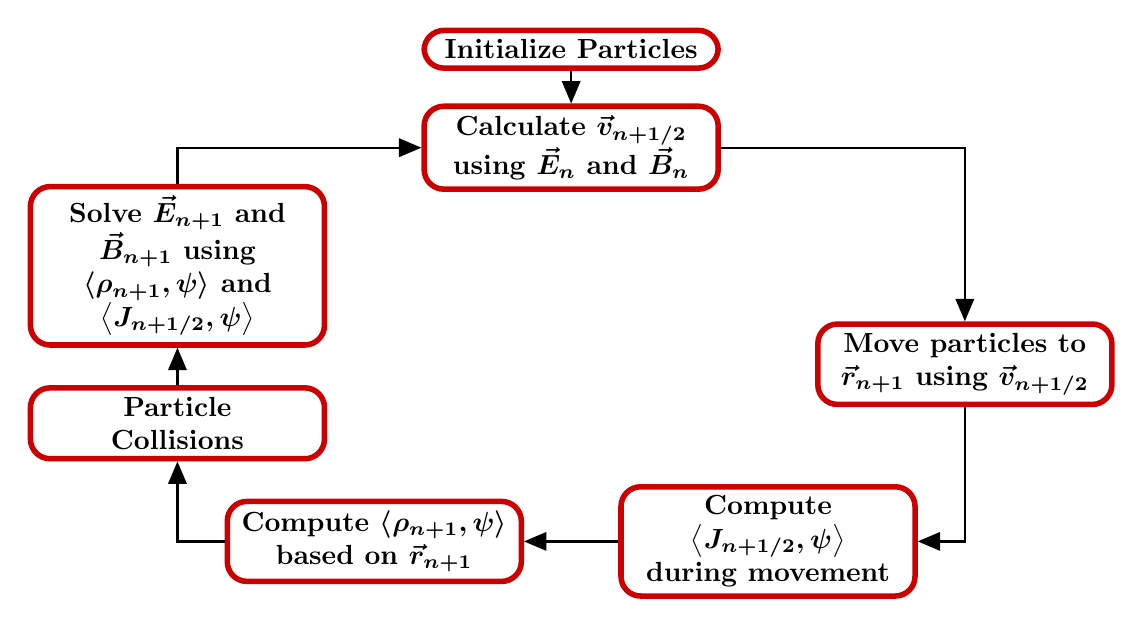
\begin{tikzpicture}[
    auto,
    node distance = 1cm,
    very thick,
    algoBlue/.style={rectangle,
    draw=NCSURed,
    font=\bfseries\boldmath,
    text width=3.5cm,
    align=center,
    rounded corners=2.5mm},
    auto,
    line width = 2pt
    ]
    \node[algoBlue] (1) [yshift=0.25cm] {Initialize Particles};
    \node[algoBlue] (2) [yshift=-1cm] {Calculate $\vec{v}_{n+1/2}$ using $\vec{E}_n$ and $\vec{B}_n$};
    \draw[line width=0.3mm, >=triangle 45, ->] (1) -- (2);
    \node[algoBlue] (3) [xshift=5cm, yshift=-3.75cm] {Move particles to $\vec{r}_{n+1}$ using $\vec{v}_{n+1/2}$};
    \draw[line width=0.3mm, >=triangle 45, ->] (2.east) -| (3.north);
    \node[algoBlue] (4) [xshift=2.5cm, yshift=-6cm] {Compute $\left< J_{n+{1/2}}, \psi \right>$ during movement};
    \draw[line width=0.3mm, >=triangle 45, ->] (3.south) |- (4.east);
    \node[algoBlue] (5) [xshift=-2.5cm, yshift=-6cm] {Compute $\left< \rho_{n+1}, \psi \right>$ based on $\vec{r}_{n+1}$};
    \draw[line width=0.3mm, >=triangle 45, ->] (4) -- (5);
    \node[algoBlue] (6)  [xshift=-5cm, yshift=-4.5cm] {Particle\\Collisions};
    \draw[line width=0.3mm, >=triangle 45, ->] (5.west) -| (6.south);
    \node[algoBlue] (7)  [xshift=-5cm, yshift=-2.5cm] {Solve $\vec{E}_{n+1}$ and $\vec{B}_{n+1}$ using $\left< \rho_{n+1}, \psi \right>$ and $\left< J_{n+{1/2}}, \psi \right>$};
    \draw[line width=0.3mm, >=triangle 45, ->] (6) -- (7);
    \draw[line width=0.3mm, >=triangle 45, ->] (7.north) |- (2.west);
  \end{tikzpicture}
\end{figure}
\end{frame}

\section{Mathematics and Verification}

\begin{frame}{Verification Motivation}
  \vfill{}
  \begin{itemize}
    \item Rigorous verification denomstrates the proper implemenation of FENIX's PIC capabilities.
    \begin{itemize}
      \item Gives researchers a higher degree of confidence when exploring new devices/regimes.
      \item Enables an easier road for licensing of designs based on FENIX calculations.
    \end{itemize}
    \item PIC is heavily utilized by the Low Temperature Plasma (LTP) community.
    \begin{itemize}
      \item Verification studies are not prioritized and are rarely published in the LTP community\cite{alves2023foundations}.
    \end{itemize}
  \end{itemize}
\end{frame}

\begin{frame}{Particle Description}
    \vfill{}
    \begin{itemize}
      \item FENIX treats computational particles as point particles.
    \end{itemize}
    \begin{align*}
      f \left( \vec{r}, \vec{v}, t \right) 
      =
      \sum_{i=1}^N 
      \omega_i q_i 
      \delta \left( \vec{r} - \vec{r}_i(t) \right)
      \delta \left( \vec{v} - \vec{v}_i(t) \right)
    \end{align*}
    \begin{columns}
      \column{0.5\textwidth}
      \begin{itemize}
        \item $f\;$: Particle distribution function.
        \item $N\;$: Computational particle count. 
        \item $\omega_i\;$: Computational particle weight.
        \item $q_i\;$: Computational particle charge.
      \end{itemize} 
      \column{0.5\textwidth}
      \begin{itemize}
        \item $\delta\;$: Dirac Delta Function.
        \item $\vec{r}\;$: Particle position.
        \item $\vec{v}\;$: Particle velocity
        \item $t\;$: Simulation time
      \end{itemize}
    \end{columns}
\end{frame}

\begin{frame}{Single Particle Motion}
  \vfill{}
  \centering
  The equations of motion are solved for each computational particle, individually.
    \centering
      \begin{equation*}
        \diff{\,\vec{r}}{t}
        =
        \vec{v}
      \end{equation*}
      \begin{equation*}
          \diff{\,\vec{v}}{t}
          =
          \frac{q}{m}
          \left(
            \vec{E} +
            \vec{v} \times
            \vec{B}
          \right)
      \end{equation*}
      \begin{itemize}
        \item $\vec{E}$ and $\vec{B}$ represent the electric and magnetic fields repsectively.
        \item The standard methods for doing this numerically are the Leapfrog method and the Boris method.
      \end{itemize}
    
\end{frame}

\begin{frame}{Leapfrog Particle Stepping}
  \vspace{1cm}
  \begin{figure}[H]
    \centering
    \includegraphics[width=\textwidth]{figs/BorisVisualization.png}
  \end{figure}
  \begin{align*}
    \vec{r}_{n+1} = \vec{r}_n + \vec{v}_{n + 1/2} \Delta t
  \end{align*}
\end{frame}


\begin{frame}{Boris Stepping}
  \vspace{1cm}
  \begin{columns}
    \column{0.5\textwidth}
    \begin{align*}
      \vec{E} = E_0 \hat{x}
    \end{align*}
    \column{0.5\textwidth}
    \begin{align*}
      \vec{B} = B_0 \hat{z}
    \end{align*}
  \end{columns} 
  \vspace{-2cm}
  \begin{columns}
    \column{0.25\textwidth}
      \begin{figure}[H]
        \centering
        \begin{tikzpicture}
          \node[above] at (1.75,2.5) {};
          \draw[line width=0.3mm, >=triangle 45, ->] (1,0) -- (2,0) node[midway, above] {$\vec{v}_n$};
            \draw[->] (0,-2) -- (0.5,-2) node[midway, right=10pt] {$x$};  % X-axis
            \draw[->] (0,-2) -- (0,-1.5) node[midway, above=10pt] {$y$};  % Y-axis
        \end{tikzpicture}
      \end{figure}
    \column{0.25\textwidth}
      \begin{figure}[H]
        \centering
        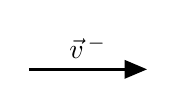
\begin{tikzpicture}
          \draw[line width=0.3mm, >=triangle 45, ->] (1,0) -- (2.5,0) node[midway, above] {$\vec{v}^{\,-}$};
        \end{tikzpicture}
      \end{figure}
    \column{0.25\textwidth}
      \begin{figure}[H]
        \centering
        \begin{tikzpicture}
          \node[above] at (1.75,1.6) {};
          \draw[line width=0.3mm, >=triangle 45, ->] (1,0) -- (2.05,-1.05 );
          \node[above] at (1.75,0) {$\vec{v}^{\,+}$};
        \end{tikzpicture}
      \end{figure}
    \column{0.25\textwidth}
      \begin{figure}[H]
        \centering
        \begin{tikzpicture}
          \node[above] at (1.75,1.6) {};
          \draw[line width=0.3mm, >=triangle 45, ->] (1,0) -- (3.5,-1.05 );
          \node[above] at (1.75,0) {$\vec{v}_{n+1}$};
        \end{tikzpicture}
      \end{figure}
  \end{columns}
  \vspace{1cm}
  \begin{columns}
    \column{0.25\textwidth}
    1: Initial Velocity at step $n$
    \column{0.25\textwidth}
    2: Accelerate with $\vec{E}$ through $\Delta t/2$
    \column{0.25\textwidth}
    3: Rotate with $\vec{B}$ through $\Delta t$
    \column{0.25\textwidth}
    4: Accelerate with $\vec{E}$ through $\Delta t/2$
  \end{columns}
%  \vfill{}
%  \centering
%  Particles are stepped through electromagnetic fields using the boris algorithm\cite{boris1970relativistic}.
%  \vspace{0.25cm}
%  \begin{columns}
%    \column{0.5\textwidth}
%      \begin{equation} \label{eq:e_half1} \vec{v}^{\,-}
%        =
%        \vec{v}_{n}
%        +
%        \frac{q}{m}
%        \vec{E}_n
%        \frac{\Delta t}{2}
%      \end{equation}
%      \begin{equation} \label{eq:boris_v_plus}
%        \vec{v}^{\,+}
%        =
%        \vec{v}^{\,-}
%        +
%        \vec{v}^{\,'}
%        \times
%        \vec{s}
%      \end{equation}
%      \begin{equation} \label{eq:boris_v_prime}
%        \vec{v}^{\,'}
%        =
%        \vec{v}^{\,-}
%        +
%        \vec{v}^{\,-}
%        \times
%        \vec{l}
%      \end{equation}
%      \begin{equation} \label{eq:boris_t}
%        \vec{l} =
%        \frac{q}{m}
%        \vec{B}_n
%        \Delta t
%      \end{equation}
%      \column{0.5\textwidth}
%      \begin{equation} \label{eq:boris_s}
%        \vec{s} =
%        \frac{2 \vec{l}}{
%          1 + \vec{l} \cdot \vec{l}
%        }
%      \end{equation}
%      \begin{equation} \label{eq:mag_step}
%        \frac{
%          \vec{v}^{\,+}
%          -
%          \vec{v}^{\,-}
%        }{ \Delta t}
%        =
%        \frac{q}{m}
%        \left(
%          \vec{v}^{\,+}
%          +
%          \vec{v}^{\,-}
%        \right)
%        \times
%        \vec{B}_n
%      \end{equation}
%      \begin{equation} \label{eq:e_half2}
%        \vec{v}_{n+1}
%        =
%        \vec{v}^{\,+}
%        +
%        \frac{q}{m}
%        \vec{E}_n
%        \frac{\Delta t}{2}
%      \end{equation}
%  \end{columns}
%  \vspace{0.25cm}
%  $\vec{E}$ and $\vec{B}$ represent the electric and magnetic fields respecitvely, and $n$ is denotes the number of the current timestep.
\end{frame}
%
\begin{frame}{Cyclotron Motion}
  \vfill{}
  \begin{columns}
    \centering
    \column{0.5\textwidth}
    \begin{itemize}
      \item A single particle in the magnetic field given by $\vec{B} =  \hat{z} \unit{T}$
      \item Particle Properties:
      \begin{itemize}
        \item $q = 1 \unit{C}$
        \item $m  = 1 \unit{kg}$ 
        \item $\omega = 1 \fracunit{1}{m}$
        \item $v_\perp = 1 \fracunit{m}{s}$
      \end{itemize}
    \end{itemize}
    $v_\perp$ is the magnitude of the velocity perpendicular to the magnetic field.
    \column{0.5\textwidth}
    \vspace{0.75cm}
    \begin{figure}[ht]
    \begin{tikzpicture}
        \node[anchor=south west,inner sep=0] (image) at (0,0) {\includegraphics[width=0.8\textwidth]{figs/cyclotron.png}};
        \begin{scope}[x={(image.south east)},y={(image.north west)}] % Coordinate system based on the image
        \draw[line width=0.5mm, >=triangle 45, ->] (0.59,0.97) arc[start angle=90, end angle=30, radius=0.39];

        %(0.59,0.95) -- (0.85,0.95); 
        % Draw aarrow from (x1, y1) to (x2, y2)
        \end{scope}
    \end{tikzpicture}
    \end{figure}
  \end{columns}
\end{frame}

\begin{frame}{Cyclotron Motion Errors}
  \vfill{}
  \begin{columns}
    \centering
    \column{0.5\textwidth}
      \begin{figure}[H]
        \includegraphics[width=0.9\textwidth]{figs/cyclotron_l2_error.png}
      \end{figure}
    \column{0.5\textwidth}
      \begin{figure}[H]
        \includegraphics[width=0.9\textwidth]{figs/cyclotron_error.png}
      \end{figure}
  \end{columns}
\end{frame}

\begin{frame}{Charge Density Calculation}
    \vspace{1cm}
    \begin{equation}
      \left< \, 
      \rho_n, 
      \psi
      \right> 
      = 
      \sum_{j=1}^{N_i} 
      q_j\,
      \omega_j\,
      \psi
      \left( \vec{r} - \vec{r}_j(t_n)
      \right) 
    \end{equation}
    \vspace{-0.25cm}
  \begin{columns}
    \column{0.5\textwidth}
    \begin{itemize}
      \item When using electrostatics the electric field can be calculated via Poisson's equation.
    \end{itemize}
    \begin{align*}
      \laplacian \phi = \frac{ \rho }{ \varepsilon_0 }
    \end{align*}
    \begin{itemize}
      \item The variational formulation requies evaluating the inner product of the computational charge distribution and the basis functions, $\psi$
    \end{itemize}
    \column{0.5\textwidth}
    \begin{figure}[H]
      \centering 
      \includegraphics[width=0.8\textwidth]{figs/charge_1D.png}
    \end{figure}
  \end{columns}
\end{frame}


\begin{frame}{Verification Problem}
  \vspace{1cm}
  \begin{columns}
    \column{0.5\textwidth}
    \begin{itemize}
      \item Represent a uniform charge density profile with computational partilces.
    \end{itemize}
    \begin{align*}
      \frac{\rho}{\varepsilon_0} = 6
      \fracunit{V}{m$^2$}
    \end{align*}
    \begin{itemize}
      \item Solve for an electric potential consistent with the charge density profile.
    \end{itemize}
    \begin{align*}
      \phi(x, y, z) 
      =x  (1 - x) + y (1 - y) + z  (1 - z) 
      \unit{V}
    \end{align*}
    \column{0.5\textwidth}
    \begin{figure}[H]
      \centering
      \includegraphics[width=0.8\textwidth]{figs/density_verification.png}
    \end{figure}
  \end{columns}
\end{frame}

\begin{frame}{Charge Density}
  \vspace{1cm}
  \begin{columns}
    \column{0.5\textwidth}
      \begin{itemize}
          \item Weights are assigned based on target number density $\rho_n$ element volume $V_E$ and particles per element, $N$.
      \end{itemize}
      \begin{align*}
        \omega = 
        \frac{\rho_n V_E}{N}
      \end{align*}
      \begin{itemize}
      \item Position are randomly sampled so the error in the projection of the density onto the mesh follows a sample variance.
      \end{itemize}
      \begin{align*}
        S^2 = 
        \frac{ 1 }{ N - 1 }
        \sum_{i=1}^N 
        \left( x_i - \overline{x} \right)^2
      \end{align*}
    \column{0.5\textwidth}
      \centering 
      \begin{figure}
        \centering 
        \includegraphics[height=0.7\textheight]{figs/density_error.png}
      \end{figure}
  \end{columns}
\end{frame}

\begin{frame}{Electrostatic Potential}
  \vfill{}
  \begin{columns}
    \column{0.5\textwidth}
    \begin{itemize}
      \item In this example first order finite element basis functions are used. 
      \begin{itemize}
        \item These basis functions have second order convergence. 
        \item Using particles as the source terms should not effect the spatial convergence rate of the system.
      \end{itemize}
    \end{itemize}
    \column{0.5\textwidth}
    \begin{figure}[H]
      \includegraphics[width=0.8\textwidth]{figs/potential_error.png}
     \end{figure}
  \end{columns}
\end{frame}

\begin{frame}{Current Density} 
    \vspace{1cm}
      \begin{align*}
        \left<
          \vec{J}_{n + 1/2}
          \left(\vec{r}, t\right),
          \vec{\psi}(\vec{r}\,)
          \right> =
        \frac{1}{\Delta t}
        \int_{t_n}^{t_{n+1}}
        \sum_{i=1}^N
        q_i \,\omega_i
        \vec{v}_i(t)
        \cdot
        \vec{\psi}(\vec{r}_i(t))
        dt
      \end{align*} 
      \vspace{-1cm}
  \begin{columns}
    \column{0.7\textwidth}
      \vspace{0.5cm}
      \begin{itemize}
        \item Time averaging the current density ensures charge conservation\stepcounter{footnote}\cite{eastwood1991virtual}$^,$\stepcounter{footnote}\cite{pinto2014charge}.
        \begin{itemize}
          \item Conservation is required to ensure Maxwell's equations are well posed.
        \end{itemize}
      \end{itemize}
      \begin{align*}
        \pdiff{\rho}{t} &= - \div \vec{J}\\
        \left< \rho_1 - \rho_0, \psi \right> &= \Delta t \left< \vec{J}_{n + 1/2}, \grad \psi \right>
      \end{align*}
    \column{0.3\textwidth}

    \begin{figure}[ht]
    \begin{tikzpicture}
        \node[anchor=south west,inner sep=0] (image) at (0,0) {\includegraphics[width=\textwidth]{figs/conservation.png}};
        \begin{scope}[x={(image.south east)},y={(image.north west)}] % Coordinate system based on the image
        \draw[line width=0.25mm, >=triangle 45, ->] (0.59,0.45) -- (0.36,0.65);
        \node[] at (0.5,-0.05) {\footnotesize$C\;/$m$^2$};
        %(0.59,0.95) -- (0.85,0.95); 
        % Draw aarrow from (x1, y1) to (x2, y2)
        \end{scope}
    \end{tikzpicture}
  \end{figure}
%    \end{figure}
%    \begin{figure}
%      \centering 
%      \includegraphics[width=1.1\textwidth]{figs/conservation.png}
%      \setlength{\unitlength}{1cm}
%      \begin{picture}(0,0)
%        \put(-0.3, 0.5){\makebox(0,0)[lt]{{\footnotesize[$C$ \textbf{/} m$^2$]}}} % Add a textbox at coordinates (2,2)
%      \end{picture}
%    \end{figure}
  \end{columns}
\end{frame}

\begin{frame}{Lieberman Benchmark}
  \vfill{}
  \begin{columns}
    \column{0.33\textwidth}
    \begin{figure}[H]
      \centering
      \includegraphics[width=\textwidth]{figs/lieberman_vdf_comparison.png}
    \end{figure}
    \column{0.33\textwidth}
    \begin{figure}[H]
      \centering
      \includegraphics[width=\textwidth]{figs/lieberman_potential_comparison.png}
    \end{figure}
    \column{0.33\textwidth}
    \begin{figure}[H]
      \centering
      \includegraphics[width=\textwidth]{figs/lieberman_population_comparison.png}
    \end{figure}
  \end{columns}
    \vspace{0.5cm}
    A simple collisionless single particle simulation demonstration from Lieberman\cite{lieberman2005} was replicated and documented as a training example.
\end{frame}

\section{Future Work}
\begin{frame}{Future Work} 
  \vfill{}
  \begin{itemize}
    \item Currently work is underway to demonstrate some canonical kinetic plasma instabilities:
    \begin{itemize}
      \item Landau Damping
      \item Two-stream instability
      \item Dory–Guest–Harris
    \end{itemize}
    \item Replication of an analytic solution applicable to both fluid and kinetic simulations\cite{lafleur2022space}.
    \item Direct Simulaiton Monte Carlo collisions will be implemented.
    \item Computing heatfluxes from particle fluxes.
    \item Coupling with other MOOSE applications.
  \end{itemize}
\end{frame}
%
\section{Summary}
\begin{frame}{Summary}
  \vfill{}
  \begin{columns}
    \column{0.5\textwidth}
    \begin{itemize}
      \item The fundamental capabilities for PIC have been verified.
      \item FENIX will enable FEM PIC simulations within the MOOSE frameowork.
      \item FENIX can perform simulations in 1D, 2D, and 3D.
      \item Rhobust verification enables FENIX to be able to utilized as an engineering tool.
      \item Once DSMC has been implemented FENIX will be capable of modeling the conditions in fusion plasma edges.
    \end{itemize}
    \column{0.5\textwidth}
    \begin{figure}[H]
      \includegraphics[width=0.7\textwidth]{figs/potential_visualiation.png}
     \end{figure}
  \end{columns}
\end{frame}
\begin{frame}
\end{frame}
%
\end{document}
